% Cread by Banbara on Dec. 19 2019
\documentclass[11pt,dvipdfmx,handout]{beamer}

%\documentclass[a4paper,12pt]{jarticle}
%\usepackage{beamerarticle}

%%%% Packages %%%%%
 \usepackage{graphicx}
% \usepackage{amsmath,amssymb,amsthm}
% \usepackage{multirow}
% \usepackage{url}
% \usepackage{tikz}
% \usepackage{alltt}
\usepackage{bm}
% \usepackage{listings,jlisting}
% \usepackage{listings}
% \lstset{
%  basicstyle=\ttfamily\scriptsize,
%  keepspaces=true,
%  escapechar=|,
%  columns=[l]{fullflexible}
% }

%%%% Fonts %%%%%
\renewcommand{\kanjifamilydefault}{\gtdefault}
% \usepackage{otf} % otfパッケージ
\usepackage[deluxe]{otf} 
\usepackage{txfonts} % 数式・英文ローマン体を Lxfont にする
% \usepackage[T1]{fontenc} % 8bit フォント
% \usepackage{minijs}
% \usepackage{textcomp} % 欧文フォントの追加
% \usepackage[utf8]{inputenc} % 文字コードをUTF-8

%%%% Beamer %%%%%
\usetheme{Madrid}
\useinnertheme{rectangles}
%\useoutertheme{smoothbars}
\setbeamercolor{enumerate}{fg=white, bg=black}
\usefonttheme{professionalfonts}
\setbeamertemplate{frametitle}[default][center]
\setbeamertemplate{navigation symbols}{}
% \setbeamercovered{transparent} % 好みに応じてどうぞ
\setbeamertemplate{footline}[frame number]
\setbeamercolor{page number in head/foot}{fg=black} % ページ数を表示する
% \setbeamerfont{footline}{size=\normalsize,series=\bfseries}
\setbeamerfont{footline}{size=\scriptsize,series=\mdseries}
\setbeamercolor{footline}{fg=black,bg=black}
\setbeamertemplate{blocks}[rounded][shadow=true]
\setbeamertemplate{items}[ball]
% \setbeamertemplate{enumerate items}[default]
% \setbeamerfont{alerted text}{series=\bfseries}

%%%% My macro %%%%%
%%%%%%%%%%%%%%%%%%%%%%%%%%%%%%%%%%%%%%%%%%%%%%%%%%%%%%%%%%%%%%%%
% User-defined Macro
%%%%%%%%%%%%%%%%%%%%%%%%%%%%%%%%%%%%%%%%%%%%%%%%%%%%%%%%%%%%%%%%
\newcommand{\compress}{\itemsep0pt\parsep0pt\parskip0pt\partopsep0pt}
% \newcommand{\compress}{\itemsep1pt plus1pt\parsep0pt\parskip0pt}
% \newcommand{\code}[1]{\lstinline[basicstyle=\ttfamily]{#1}}
\newcommand{\gringo}{\textit{gringo}}
\newcommand{\clasp}{\textit{clasp}}
\newcommand{\clingo}{\textit{clingo}}
\newcommand{\teaspoon}{\textit{teaspoon}}
\newcommand{\sat}{\textsf{SAT}}
\newcommand{\unsat}{\textsf{UNSAT}}
% \newcommand{\web}[2]{\href{#1}{#2\ \raisebox{-0.15ex}{\beamergotobutton{Web}}}}
% \newcommand{\doi}[2]{\href{#1}{#2\ \raisebox{-0.15ex}{\beamergotobutton{DOI}}}}
% \newcommand{\weblink}[1]{\web{#1}{#1}}
% \newcommand{\imp}{\mathrel{\Rightarrow}}
% \newcommand{\Iff}{\mathrel{\Leftrightarrow}}
% \newcommand{\mybox}[1]{\fbox{\rule[.2cm]{0cm}{0cm}\mbox{${#1}$}}}
% \newcommand{\mycbox}[2]{\tikz[baseline]\node[fill=#1!10,anchor=base,rounded corners=2pt] () {#2};}
% \newcommand{\naf}[1]{\ensuremath{{\sim\!\!{#1}}}}
% \newcommand{\head}[1]{\ensuremath{\mathit{head}(#1)}}
% \newcommand{\body}[1]{\ensuremath{\mathit{body}(#1)}}
% \newcommand{\atom}[1]{\ensuremath{\mathit{atom}(#1)}}
% \newcommand{\poslits}[1]{\ensuremath{{#1}^+}}
% \newcommand{\neglits}[1]{\ensuremath{{#1}^-}}
% \newcommand{\pbody}[1]{\poslits{\body{#1}}}
% \newcommand{\nbody}[1]{\neglits{\body{#1}}}
% \newcommand{\Cn}[1]{\ensuremath{\mathit{Cn}(#1)}}
% \newcommand{\reduct}[2]{\ensuremath{#1^{#2}}}
% \newcommand{\OK}{\mbox{\textcolor{green}{\Pisymbol{pzd}{52}}}}
% \newcommand{\KO}{\mbox{\textcolor{red}{\Pisymbol{pzd}{56}}}}
% \newcommand{\code}[1]{\lstinline[basicstyle=\ttfamily]{#1}}
% \newcommand{\lw}[1]{\smash{\lower2.ex\hbox{#1}}}
\newcommand{\llw}[1]{\smash{\lower3.ex\hbox{#1}}}

\newenvironment{tableC}{%
  \scriptsize
  \renewcommand{\arraystretch}{0.9}
  \tabcolsep = 0.6mm
  % \begin{tabular}[t]{p{6mm}|rlr|rlr|rlr|rlr|rlr}\hline
  %   \multicolumn{1}{l|}{\llw{問題   }} &
  \begin{tabular}[t]{l|rlr|rlr|rlr|rlr|rlr}\hline
    \multicolumn{1}{l|}{\llw{問題}} &
    \multicolumn{3}{c|}{UD1} &
    \multicolumn{3}{c|}{UD2} &
    \multicolumn{3}{c|}{UD3} &
    \multicolumn{3}{c|}{UD4} &
    \multicolumn{3}{c}{UD5} \\
    & 
    \multicolumn{1}{c}{既知の} & & \multicolumn{1}{c|}{ASP} & 
    \multicolumn{1}{c}{既知の} & & \multicolumn{1}{c|}{ASP} & 
    \multicolumn{1}{c}{既知の} & & \multicolumn{1}{c|}{ASP} & 
    \multicolumn{1}{c}{既知の} & & \multicolumn{1}{c|}{ASP} & 
    \multicolumn{1}{c}{既知の} & & \multicolumn{1}{c}{ASP} \\
    & 
    ベスト & &  & 
    ベスト & &  & 
    ベスト & &  & 
    ベスト & &  & 
    ベスト & &  \\
    \hline
  }{%
    \hline
  \end{tabular}
}

%%%%%%%%%%%%%%%%%%%%%%%%%%%%%%%%%%%%%%%%%%%%%%%%%%%%%%%%%%%%%%%%%%%%%%%
\title{解集合プログラミングを用いた\\時間割問題の解法に関する考察}
\author{桑原 和也}
%\institute{名古屋大学工学部電気電子・情報学科情報コース}
\date{2019年度卒業研究発表会\\2020年2月20日}
\institute{番原研究室}
\begin{document}
\maketitle
%%%%%%%%%%%%%%%%%%%%%%%%%%%%%%%%%%%%%%%%%%%%%%%%%%%%%%%%%%%%%%%%%%%%%%%
\begin{frame}{時間割問題}
  \begin{block}{}\centering
    求解困難な組合せ最適化問題の一種である.
  \end{block}
  \begin{itemize}
    % \item 現状では,実行可能で質の高い時間割を作成するために
    %   多くの人間の労力が費やされている.
  \item 時間割に関する国際会議 PATAT および
    \alert{\bf 国際的な時間割競技会}が開催され,
    時間割ソルバーの性能向上に貢献している.
    \begin{itemize}
    \item 教育時間割
      \begin{itemize}
      \item \alert{\bf カリキュラムベース・コース時間割 (CB-CTT)}
      \item ポストエンロールメント・コース時間割
      \item 試験時間割
      \end{itemize}
    \item 輸送時間割
    \item 従業員時間割
    \item スポーツ時間割
    \end{itemize}
  \item 本発表では,最も研究が盛んな CB-CTT を対象とする.
  \item CB-CTT は,以下のように定式化される.
    \begin{itemize}
    \item 必ず満たすべき\structure{\bf ハード制約}と, 
    できるだけ満たしたい\structure{\bf 重み付きソフト制約}から構成される.
    \item 違反するソフト制約の重み (ペナルティ) の総和の最小化が目的.
    \end{itemize}
  \end{itemize}
\end{frame}
%%%%%%%%%%%%%%%%%%%%%%%%%%%%%%%%%%%%%%%%%%%%%%%%%%%%%%%%%%%%%%%%%%%%%%%
\begin{frame}{解集合プログラミング(Answer Set Programming; ASP)}
  \begin{itemize}
  \item \structure{\bf ASP言語}は,一階論理に基づく知識表現言語の一種である.
  \item \structure{\bf ASPシステム}は,安定モデル意味論~[Gelfond and Lifschitz '88]
    に基づく解集合を計算するシステムである.
  \item 近年,SAT技術を利用した高速なASPシステムが開発され,ロボット工学,
    システム検証,システム生物学など
    様々な分野への実用的応用が急速に拡大している.
  \end{itemize}
  \begin{alertblock}{組合せ最適化問題に対してASPを用いる利点}
    \begin{itemize}
 %   \item ASP言語の高い表現力により,各制約を表現する論理プログラムを
 %    モジュール化して容易に切り替え可能である.
    \item ASP言語の高い表現力により,記号的制約を簡潔に記述できる.
    \item 系統的探索 (分枝限定法) なので,解の最適性を保証できる.
%    \item 様々な最適化手法や探索ヒューリスティックスを試せる.
    \item 探索ヒューリスティックスを試せる.
      \begin{itemize}
      \item 探索時に優先的に割り当てる値を指定できる.
      \end{itemize}
  %  \item Python インターフェースを利用して,メタヒューリスティックスを実装できる.
    \end{itemize}
  \end{alertblock}
\end{frame}
%%%%%%%%%%%%%%%%%%%%%%%%%%%%%%%%%%%%%%%%%%%%%%%%%%%%%%%%%%%%%%%%%%%%%%%
\begin{frame}{CB-CTT に対する既存ASP解法の問題点}
  \begin{itemize}
  \item ASP による CB-CTT の解法は,
    最も成功した ASP 応用事例の一つとして知られている~[Banbara+ '13, '16, '18].
    \begin{itemize}
    \item ベンチマーク問題305問のうち,
      182問で既知の最良値と同じかより良い値が求められている.
    \end{itemize}
  \item 系統的探索であることを活かして,最適値が未知であった51問の問題で最適値決定にも成功している.
 %   \begin{itemize}
 %   \item 305問中51問で最適値が求められている.
 %   \end{itemize}
  \end{itemize}
  \begin{alertblock}{既存ASP解法の問題点}
    \begin{itemize}
    \item ソフト制約が多く含まれるような問題集において,
      局所的探索より性能が劣っている場合がみられる.
     \item 既知の最良値との比の平均値は
       \begin{itemize}
       \item ソフト制約が少ない問題集 (UD1) では $+19.83\%$
       \item ソフト制約が多い問題集 (UD5) では $+100.17\%$
       \end{itemize}
    \end{itemize}
  \end{alertblock}
\end{frame}
%%%%%%%%%%%%%%%%%%%%%%%%%%%%%%%%%%%%%%%%%%%%%%%%%%%%%%%%%%%%%%%%%%%%%%%
%%%%%%%%%%%%%%%%%%%%%%%%%%%%%%%%%%%%%%%%%%%%%%%%%%%%%%%%%%%%%%%%%%%%%%%
\begin{frame}{研究目的}
  \begin{exampleblock}{先行研究}
    \begin{itemize}
    \item 系統的探索と局所的探索を組み合わせた
      \alert{優先度付き大域近傍探索 (LNPS)} [坡山ほか '18]
      が提案されている.
    \item LNPSは,暫定解に含まれる変数の値割り当ての一部をランダムに選んで取り
      消し(\alert{destroy}),他の値割り当てをなるべく維持したままで解を
      再探索する方法である.
    \end{itemize}
  \end{exampleblock}

  \begin{alertblock}{研究目的}
    LNPSをASP上に実装し,CB-CTT に適用・評価する.
  \end{alertblock}

  \begin{block}{研究内容}
    \begin{enumerate}
    \item LNPS の性能に重要な役割を果たす destroy 演算について,
      CB-CTT に適した3種類の手法の実装. 
    \item CB-CTT に対する実験・評価
    \end{enumerate}
  \end{block}
\end{frame}
%%%%%%%%%%%%%%%%%%%%%%%%%%%%%%%%%%%%%%%%%%%%%%%%%%%%%%%%%%%%%%%%%%%%%%%

%%% Local Variables:
%%% mode: latex
%%% TeX-master: slide
%%% End:

%%%%%%%%%%%%%%%%%%%%%%%%%%%%%%%%%%%%%%%%%%%%%%%%%%%%%%%%%%%%%%%%%%%%%%%%
\begin{frame}{研究目的}

  \begin{alertblock}{研究目的}
    系統的探索と局所的探索を組み合わせた
    \alert{Large Neighborhood Prioritized Search (LNPS)} [坡山ほか '18]
    をASP上に実装し,CB-CTT に適用・評価する.
    LNPSは,暫定解に含まれる変数の値割り当ての一部をランダム
    に選んで取り消し,他の値割り当てをなるべく維持したままで
    解を再構築する反復法の一種である.
  \end{alertblock}

  \begin{block}{研究内容}
    \begin{enumerate}
    \item LNPS の性能に重要な役割を果たす destroy 演算について,
      CB-CTT に適した3種類の手法
       (random, day-period, day-room)
      を実装した. 
      \begin{itemize}
      \item randomは問題の性質を利用しない手法.
      \item day-period, day-roomはCB-CTTのソフト制約を考慮した手法.
      \end{itemize}
    \item CB-CTT に対する実験・評価
    \end{enumerate}
  \end{block}
\end{frame}
%%%%%%%%%%%%%%%%%%%%%%%%%%%%%%%%%%%%%%%%%%%%%%%%%%%%%%%%%%%%%%%%%%%%%%%

%%%%%%%%%%%%%%%%%%%%%%%%%%%%%%%%%%%%%%%%%%%%%%%%%%%%%%%%%%%%%%%%%%%%%%%
\begin{frame}{LNPS: 優先度付き大域近傍探索 [坡山'18]}
  \begin{block}{\small LNPS のアルゴリズム}
    \begin{enumerate}
      \compress
      \item 初期解を $x$ と置き,最良解 $x* := x$ とする.
      \item 以下の destroy と re-searchで $x$ から得られた解を $x_t$ と置く.
      \begin{itemize}
        \compress
        \item \alert{\bf destroy} は $x$ から値割当ての一部を\structure{取り消し} $x'$ とする.
        \item re-search は $x'$ の値割当てをなるべく維持したまま再探索する.
      \end{itemize}
      \item 更新条件を満たしていたら $x := x_t$ とする.
      \begin{itemize}
        \item 例えば「$x_t$ が $x$ より改善された解なら」という更新条件を用いる.
      \end{itemize}
      \item $x_t$ が最良解 $x*$ より改善された解なら,$x* := x_t$ とする.
      \item 終了条件が満たされるまで,2〜4 を繰り返す.
      \begin{itemize}
        \item 例えば繰り返し回数や制限時間などを終了条件に用いる.
      \end{itemize}
      \item 最良解 $x*$ を返す.
    \end{enumerate}
  \end{block}

  % \begin{itemize}
  % % \item 運搬経路問題 (Vehicle Routing Problem)
  % %  等に対して有効性が示されている
  % %  Large Neighborhood Search (LNS) [Shaw '98, Ropke and Pisinger '10]
  % %  をベース
  % \end{itemize}
  \begin{alertblock}{}\centering
    問題に応じて,\alert{\bf 適切な destroy 演算を設計}することが重要
  \end{alertblock}
\end{frame}
%%%%%%%%%%%%%%%%%%%%%%%%%%%%%%%%%%%%%%%%%%%%%%%%%%%%%%%%%%%%%%%%%%%%%%%
\begin{frame}{実装した destroy 演算 (提案)}
  \begin{itemize}
  \item CB-CTT に関する既存研究[Kieferほか'16]を参考に,
    3種類のdestroy演算を実装した.
  \end{itemize}

  \begin{block}{}
    \begin{enumerate}
    \item \structure{\bf random $N$}
      \begin{itemize}
      \item 暫定解から値割当ての$N$\%をランダムに取り消す.
      \end{itemize}
    \item \structure{\bf day-period}
      \begin{itemize}
      \item ランダムに曜日($D$)と時限($P$)を選び,
        暫定解から$D$曜$P$限の値割当てをすべて取り消す.
      \item 教室に関するソフト制約のペナルティを減らすことが狙い.
   \end{itemize}
  \item \structure{\bf day-room}
   \begin{itemize}
   \item ランダムに曜日($D$)と教室($R$)を選び,
     暫定解から$D$曜日の$R$教室の値割当てをすべて取り消す.
   \item 時限に関するソフト制約のペナルティを減らすことが狙い.
   \end{itemize}
  \end{enumerate}
  \end{block}
 \end{frame}
%%%%%%%%%%%%%%%%%%%%%%%%%%%%%%%%%%%%%%%%%%%%%%%%%%%%%%%%%%%%%%%%%%%%%%%
\begin{frame}{実験概要}
  \begin{itemize}
  \item 提案手法の有効性を評価するために比較実験を行った.
    \begin{itemize}
    \item 既存ASP~[Banbara+ '18]
    \item 提案手法
      \begin{itemize}
      \item \structure{\bf R-\bm{$N$}}: LNPS + random $N$ ($N=0, 10, 20$)
      \item \structure{\bf DP}: LNPS + day-period
      \item \structure{\bf DR}: LNPS + day-room
      \end{itemize}
    \end{itemize}
  \item CB-CTTベンチマーク問題 (全21問)
    \begin{itemize}
    \item ソフト制約が多い問題集 (UD5) を用いる.
    \end{itemize}
  \item ASP システム:\textit{clingo-5.4.0}
  \item 制限時間 : 1時間/問
  \item 実験環境 : Mac mini (CPU : Intel Core i7 3.2GHz, メモリー : 64GB) 
  \end{itemize}
\end{frame}
%%%%%%%%%%%%%%%%%%%%%%%%%%%%%%%%%%%%%%%%%%%%%%%%
\newenvironment{tableA}{%
%  \scriptsize
%  \tabcolsep = 2mm
  \renewcommand{\arraystretch}{0.85}
  \begin{tabular}[t]{c||r|r|r|r|r|r}
    \lw{問題名} & \lw{既存ASP} & \multicolumn{5}{c}{提案手法}\\\cline{3-7}
     &  & R-0 & R-10 & R-20 & DP & DR\\\hline
    }{%
    \hline
  \end{tabular}
}

\newenvironment{tableB}{%
%  \scriptsize
  \tabcolsep = 2mm
  \renewcommand{\arraystretch}{0.815}						
  \begin{tabular}[t]{c||r|r|r|r|r|r|}\hline
    Instance & 既存ASP解法 & R-0 & R-10 & R-20 & R-dp & R-dr \\\hline
    }{%
    \hline
  \end{tabular}
}
%%%%%%%%%%%%%%%%%%%%%%% 
\begin{frame}{実験結果 : 得られた最適値・最良値}

\begin{table}[tbp]\scriptsize
  \label{table:bench:result1}
  \centering
  \begin{tableA}
    \code{comp01} & 132$^\mathrm{b}$ & 13$^\mathrm{b}$ & \bf 11$^\mathrm{\bf b}$ & \bf 11$^\mathrm{\bf b}$ & 13$^\mathrm{b}$ & \bf 11$^\mathrm{\bf b}$\\
\code{comp02} & \bf 331$^\mathrm{\bf u}$ & 455$^\mathrm{b}$ & 413$^\mathrm{b}$ & 883$^\mathrm{u}$ & 413$^\mathrm{b}$ & 387$^\mathrm{b}$\\
\code{comp03} & 302$^\mathrm{u}$ & 200$^\mathrm{u}$ & 211$^\mathrm{u}$ & 1009$^\mathrm{u}$ & \bf 187$^\mathrm{\bf u}$ & 196$^\mathrm{u}$\\
\code{comp04} & \bf 49$^\mathrm{\bf u}$ & \bf 49$^\mathrm{\bf u}$ & \bf 49$^\mathrm{\bf u}$ & \bf 49$^\mathrm{\bf u}$ & \bf 49$^\mathrm{\bf u}$ & \bf 49$^\mathrm{\bf u}$\\
\code{comp05} & 1940$^\mathrm{u}$ & 1135$^\mathrm{u}$ & 1312$^\mathrm{u}$ & 2071$^\mathrm{u}$ & \bf 1012$^\mathrm{\bf u}$ & 1109$^\mathrm{u}$\\
\code{comp06} & 822$^\mathrm{b}$ & 365$^\mathrm{b}$ & 923$^\mathrm{u}$ & 1039$^\mathrm{u}$ & 394$^\mathrm{b}$ & \bf 310$^\mathrm{\bf b}$\\
\code{comp07} & 924$^\mathrm{b}$ & 513$^\mathrm{u}$ & 1075$^\mathrm{b}$ & 1263$^\mathrm{b}$ & \bf 428$^\mathrm{\bf b}$ & 530$^\mathrm{u}$\\
\code{comp08} & \bf 55$^\mathrm{\bf u}$ & \bf 55$^\mathrm{\bf u}$ & \bf 55$^\mathrm{\bf u}$ & \bf 55$^\mathrm{\bf u}$ & \bf 55$^\mathrm{\bf u}$ & \bf 55$^\mathrm{\bf u}$\\
\code{comp09} & 254$^\mathrm{u}$ & 192$^\mathrm{u}$ & \bf 176$^\mathrm{\bf u}$ & 703$^\mathrm{u}$ & 181$^\mathrm{u}$ & 232$^\mathrm{b}$\\
\code{comp10} & 822$^\mathrm{b}$ & 377$^\mathrm{b}$ & 837$^\mathrm{b}$ & 1111$^\mathrm{b}$ & 376$^\mathrm{b}$ & \bf 367$^\mathrm{\bf b}$\\
\code{comp11} & \bf 0$^\mathrm{\bf u}$ & \bf 0$^\mathrm{\bf u}$ & \bf 0$^\mathrm{\bf u}$ & \bf 0$^\mathrm{\bf b/u}$ & \bf 0$^\mathrm{\bf u}$ & \bf 0$^\mathrm{\bf b/u}$\\
\code{comp12} & 1246$^\mathrm{u}$ & 788$^\mathrm{u}$ & 1895$^\mathrm{b}$ & 2353$^\mathrm{b}$ & 794$^\mathrm{u}$ & \bf 778$^\mathrm{\bf u}$\\
\code{comp13} & 301$^\mathrm{u}$ & 187$^\mathrm{u}$ & 241$^\mathrm{u}$ & 800$^\mathrm{b}$ & \bf 181$^\mathrm{\bf u}$ & 182$^\mathrm{u}$\\
\code{comp14} & \bf 67$^\mathrm{\bf u}$ & 72$^\mathrm{u}$ & 71$^\mathrm{u}$ & 826$^\mathrm{u}$ & 71$^\mathrm{u}$ & 72$^\mathrm{u}$\\
\code{comp15} & 607$^\mathrm{u}$ & 316$^\mathrm{u}$ & 469$^\mathrm{b}$ & 848$^\mathrm{b}$ & \bf 238$^\mathrm{\bf u}$ & 259$^\mathrm{u}$\\
\code{comp16} & 944$^\mathrm{b}$ & 416$^\mathrm{b}$ & 912$^\mathrm{b}$ & 996$^\mathrm{b}$ & \bf 356$^\mathrm{\bf b}$ & 402$^\mathrm{b}$\\
\code{comp17} & 412$^\mathrm{u}$ & 232$^\mathrm{u}$ & 328$^\mathrm{u}$ & 1018$^\mathrm{b}$ & 230$^\mathrm{u}$ & \bf 227$^\mathrm{\bf u}$\\
\code{comp18} & 471$^\mathrm{u}$ & 201$^\mathrm{b}$ & 194$^\mathrm{u}$ & 599$^\mathrm{b}$ & 222$^\mathrm{u}$ & \bf 181$^\mathrm{\bf u}$\\
\code{comp19} & 890$^\mathrm{b}$ & 331$^\mathrm{b}$ & 330$^\mathrm{u}$ & 768$^\mathrm{b}$ & 304$^\mathrm{b}$ & \bf 248$^\mathrm{\bf b}$\\
\code{comp20} & 1386$^\mathrm{u}$ & \bf 755$^\mathrm{\bf u}$ & 1374$^\mathrm{u}$ & 1546$^\mathrm{b}$ & 787$^\mathrm{u}$ & 768$^\mathrm{u}$\\
\code{comp21} & 310$^\mathrm{u}$ & 187$^\mathrm{u}$ & \bf 168$^\mathrm{\bf u}$ & 911$^\mathrm{b}$ & 178$^\mathrm{u}$ & 170$^\mathrm{u}$\\\hline
\code{最適値の数} & 4 & 3 & 3 & 3 & 3 & 3\\
\code{最良値の数} & 1 & 1 & 3 & 1 & 6 & 7\\
  \end{tableA}
\end{table}
\begin{itemize}
\item 提案手法の DP と DR が良い性能を示した.
\end{itemize}
\end{frame}
%%%%%%%%%%%%%%%%%%%%%%%%%%%%%%%%%%%%%%%%%%%%%%%%%%%%%%%%%%%%%%%%%%%%%%%
\begin{frame}{比較結果 : 既知の最良値を1とした場合の比}
\begin{table}[tbp]\scriptsize
  \label{table:bench:result2}
  \centering
  \begin{tableA}
    {comp01} & 12.00 & 1.18 & \alert{\bf 1.00} & \alert{\bf 1.00} & 1.18 & \alert{\bf 1.00} \\
{comp02} & \alert{\bf 2.54} & 3.50 & 3.17 & 6.79 & 3.17 & 2.97 \\
{comp03} & 2.12 & 1.40 & 1.48 & 7.10 & \alert{\bf 1.31} & 1.38 \\
{comp04} & \alert{\bf 1.00} & \alert{\bf 1.00} & \alert{\bf 1.00} & \alert{\bf 1.00} & \alert{\bf 1.00} & \alert{\bf 1.00} \\
{comp05} & 3.40 & 1.99 & 2.30 & 3.63 & \alert{\bf 1.77} & 1.94 \\
{comp06} & 9.67 & 4.29 & 10.85 & 12.22 & 4.63 & \alert{\bf 3.64} \\
{comp07} & 22.00 & 12.21 & 25.59 & 30.07 & \alert{\bf 10.19} & 12.61 \\
{comp08} & \alert{\bf 1.00} & \alert{\bf 1.00} & \alert{\bf 1.00} & \alert{\bf 1.00} & \alert{\bf 1.00} & \alert{\bf 1.00} \\
{comp09} & 1.69 & 1.28 & \alert{\bf 1.17} & 4.68 & 1.20 & 1.54 \\
{comp10} & 11.41 & 5.23 & 11.62 & 15.43 & 5.22 & \alert{\bf 5.09} \\
{comp11} & \alert{\bf 1.00} & \alert{\bf 1.00} & \alert{\bf 1.00} & \alert{\bf 1.00} & \alert{\bf 1.00} & \alert{\bf 1.00} \\
{comp12} & 2.57 & 1.63 & 3.92 & 4.87 & 1.64 & \alert{\bf 1.61} \\
{comp13} & 2.04 & 1.27 & 1.63 & 5.44 & \alert{\bf 1.23} & \alert{\bf 1.23} \\
{comp14} & \alert{\bf 1.00} & 1.07 & 1.05 & 12.32 & 1.05 & 1.07 \\
{comp15} & 3.44 & 1.79 & 2.66 & 4.81 & \alert{\bf 1.35} & 1.47 \\
{comp16} & 9.83 & 4.33 & 9.50 & 10.37 & \alert{\bf 3.70} & 4.18 \\
{comp17} & 2.65 & 1.49 & 2.11 & 6.56 & 1.48 & \alert{\bf 1.46} \\
{comp18} & 3.43 & 1.46 & 1.41 & 4.37 & 1.62 & \alert{\bf 1.32} \\
{comp19} & 7.12 & 2.64 & 2.64 & 6.14 & 2.43 & \alert{\bf 1.98} \\
{comp20} & 11.17 & \alert{\bf 6.08} & 11.08 & 12.46 & 6.34 & 6.19 \\
{comp21} & 2.05 & 1.23 & \alert{\bf 1.11} & 6.03 & 1.17 & 1.12 \\\hline
{平均} & 5.39 & 2.72 & 4.63 & 7.49 & \alert{\bf 2.56} & 2.61\\

  \end{tableA}
\end{table}
\begin{itemize}
\item 提案手法の DP と DR が,既知の最良値により近い解を生成
\end{itemize}\end{frame}
%%%%%%%%%%%%%%%%%%%%%%%%%%%%%%%%%%%%%%%%%%%%%%%%%%%%%%%%%%%%%%%%%%%%%%%
\begin{frame}{まとめ}
優先度付き大域近傍探索(LNPS)をASP上に実装し,CB-CTT に適用・評価した.
\begin{enumerate}
\item CB-CTTに対する3種類のdestroy演算を実装
  \begin{itemize}
  \item ASPの\texttt{\#heuristic}宣言を用いて簡潔に実装できることを確認
  \end{itemize}
\item  CB-CTTのソフト制約が多い問題集(UD5)での実験・評価
  \begin{itemize}
  \item  提案手法は,既存ASP解法と比較して, 
  21問中19問で同じかより良い解を得ることができ, 提案手法の有効性が確認できた.
  \item 問題の性質を利用した destroy 演算(day-period と day-room)
    が良い性能を示した.
  \end{itemize}
\end{enumerate}
    
\begin{alertblock}{今後の課題}
  \begin{itemize}
  \item 新しい destroy演算の考案
    \begin{itemize}
    \item 暫定解から違反の原因となる値割当てを取り消す方法
    \end{itemize}
  \item アダプティブなLNPS
    \begin{itemize}
    \item 複数のdestroy演算を動的に切換える方法の考案
    \end{itemize}
  \item 他の時間割問題への適用
    % \begin{itemize}
   % \item \footnotesize 問題のサイズによる適切なdestroyの割合の決定
   %\item \footnotesize 問題のサイズによらないdestroy演算の実装
    %\end{itemize}
    %\item 実装したdestroy演算が意図通りの働きをしているかの検証
  % \item destroy演算を組み合わせる手法の考案・評価
  % \item 他の時間割問題,および組合せ最適化問題での実験
  \end{itemize}
\end{alertblock}
\end{frame}
%%%%%%%%%%%%%%%%%%%%%%%%%%%%%%%%%%%%%%%%%%%%%%%%%%%%%%%%%%%%%%%%%%%%%%%
% 補助スライド
\appendix
%%%%%%%%%%%%%%%%%%%%%%%%%%%%%%%%%%%%%%%%%%%%%%%%%%%%%%%%%%%%%%%%%%%%%%%
\begin{frame}{制約と問題集 (カリキュラムベース・コース時間割)}
  % \begin{itemize}
  % \item \structure{シナリオ}とはソフト制約の集合である.
  %   % \item ITC2007競技会ではUD2が使用された.
  % \end{itemize}
  \begin{block}{}\small
    \begin{center}
      \begin{tabular}{l|ccccc}%\hline
        制約                      &  UD1  &  UD2  &  UD3  &  UD4  &  UD5  \\
        \hline
        $H_1$. Lectures           &  H    &  H    &  H    &  H    &  H    \\
        $H_2$. Conflicts          &  H    &  H    &  H    &  H    &  H    \\
        $H_3$. RoomOccupancy      &  H    &  H    &  H    &  H    &  H    \\
        $H_4$. Availability       &  H    &  H    &  H    &  H    &  H    \\
        $S_1$. RoomCapacity       &  1    &  1    &  1    &  1    &  1    \\
        $S_2$. MinWorkingDays     &  5    &  5    &  -    &  1    &  5    \\
        $S_3$. IsolatedLectures   &  1    &  2    &  -    &  -    &  1    \\
        $S_4$. Windows            &  -    &  -    &  4    &  1    &  2    \\
        $S_5$. RoomStability      &  -    &  1    &  -    &  -    &  -    \\
        $S_6$. StudentMinMaxLoad  &  -    &  -    &  2    &  1    &  2    \\
        $S_7$. TravelDistance     &  -    &  -    &  -    &  -    &  2    \\
        $S_8$. RoomSuitability    &  -    &  -    &  3    &  H    &  -    \\
        $S_9$. DoubleLectures     &  -    &  -    &  -    &  1    &  -  
      \end{tabular}
    \end{center}
  \end{block}
\end{frame}
%%%%%%%%%%%%%%%%%%%%%%%%%%%%%%%%%%%%%%%%%%%%%%%%%%%%%%%%%%%%%%%%
\begin{frame}{教室に関するソフト制約}
 \begin{block}{}
 \begin{itemize}
  \item \structure{\bf day-period}
   \begin{itemize}
    \item ランダムに曜日($D$)と時限($P$)を選び,
    暫定解から$D$曜$P$限の値割当てをすべて取り消す.
    \item 教室に関するソフト制約のペナルティを減らすことが狙い.
   \end{itemize}
  \end{itemize}
 \end{block}
 \begin{enumerate}
  \item \alert{RoomCapacity}
   \begin{itemize}
    \item 各科目について, 受講者数が使用する教室の収容可能人数を超えてはいけない. 
    違反した場合, 超過人数に応じたペナルティが課される. 
   \end{itemize}
  \item RoomStability
   \begin{itemize}
    \item 同一科目のすべての講義は, 同一教室で開講される. 
    違反した場合, 異なる教室数 (最初の教室は除く) に応じたペナルティが課される.
   \end{itemize}
  \item \alert{TravelDistance}
   \begin{itemize}
    \item 各課程について, 同一曜日に異なる建物の教室で開講される連続した講義が
    あると違反となり, 建物間の移動毎にペナルティが課される.
   \end{itemize}
  \item RoomSuitability
   \begin{itemize}
    \item 各科目の講義は, 開講不可能な教室で開講されることはない. 
    違反した講義毎にペナルティが課される. 
   \end{itemize}
 \end{enumerate}
\end{frame}
%%%%%%%%%%%%%%%%%%%%%%%%%%%%%%%%%%%%%%%%%%%%%%%%%%%%%%%%%%%%%%%
\begin{frame}{時限に関するソフト制約}
 \begin{block}{}
 \begin{itemize}
  \item \structure{\bf day-room}
   \begin{itemize}
    \item ランダムに曜日($D$)と教室($R$)を選び,
    暫定解から$D$曜日の$R$教室の値割当てをすべて取り消す.
    \item 時限に関するソフト制約のペナルティを減らすことが狙い.
   \end{itemize}
  \end{itemize}
 \end{block}
 \begin{enumerate}
  \item \alert{IsolatedLectures}
   \begin{itemize}
    \item  同一課程に属する講義は, 連続した時限に開講される. 
    同一曜日に同一課程に属する他のどの講義とも隣接していない (孤立した) 講義が
    ある場合に違反となり, 孤立した講義毎にペナルティが課される.
    \end{itemize}
  \item \alert{Windows}
   \begin{itemize}
    \item 同一課程に属する講義は, 空き時限なしで開講される. 
    同一曜日に同一課程に属する2つの講義の間に空き時限が
    ある場合に違反となり, 空き時限の長さに応じたペナルティが課される.   
    \end{itemize}
  \item DoubleLectures
   \begin{itemize}
    \item 連続講義の形態をとる科目は, 同一曜日に複数の講義がある場合, 
    それらは連続した時限に同一教室で開講される. 
    違反した講義毎にペナルティが課される.   
    \end{itemize}
 \end{enumerate}
\end{frame}
%%%%%%%%%%%%%%%%%%%%%%%%%%%%%%%%%%%%%%%%%%%%%%%%%%%%%%%%%%%%%%%
\begin{frame}{day-periodによるdestroy}
 \begin{block}{}
 \begin{itemize}
  \item \structure{\bf day-period}
   \begin{itemize}
    \item ランダムに曜日($D$)と時限($P$)を選び,
    暫定解から$D$曜$P$限の値割当てをすべて取り消す.
    \item 教室に関するソフト制約のペナルティを減らすことが狙い.
   \end{itemize}
  \end{itemize}
 \end{block}
  \begin{exampleblock}{}\scriptsize
    \begin{center}
     \begin{tabular}{c}
      \begin{minipage}{5.4cm}
       \begin{center}        
        \begin{tabular}{c|l|c}%\hline
                     &~~~~~~~~~~~~~1時限目& ... \\\cline{1-3}
         \vdots  &                                          &   \\\cline{1-3}
                     &  \structure{教室A : アルゴリズム}     & \\
       水曜日  &  \structure{教室B : コンパイラ}         &   \\
                    &  \structure{教室C : プログラミング}   &  \\\cline{1-3}
       \vdots &                                          &  \\
        \end{tabular}
      \end{center}
     \end{minipage}    
     \begin{minipage}{4.1cm}
      \begin{center}
       \begin{tabular}{rl}%\hline
       収容人数 : & \alert{教室A~~30人}\\
       & 教室B~~50人\\
       & 教室C~~70人\\
       受講者数 : & \alert{アルゴリズム 60人}\\
       & コンパイラ 40人\\
       & プログラミング 30人\\
      \end{tabular}
     \end{center}
    \end{minipage}    
   \end{tabular}
   \end{center}
  \end{exampleblock}
  \begin{itemize}
   \item \small destroy で曜日として水曜日, 時限として1限を選ぶとする. 
   \item \small 同一曜日, 同一時限の講義間での教室の交換を促すことで, 
   教室に関するソフト制約違反の改善を狙う. 
   \begin{itemize}
    \item アルゴリズムとプログラミングの教室を
    交換することで, 収容人数オーバーを改善することができる. 
   \end{itemize}
  \end{itemize}
\end{frame}
%%%%%%%%%%%%%%%%%%%%%%%%%%%%%%%%%%%%%%%%%%%%%%%%%%%%%%%%%
\begin{frame}{day-roomによるdestroy}
 \begin{block}{}
 \begin{itemize}
  \item \structure{\bf day-room}
   \begin{itemize}
    \item ランダムに曜日($D$)と教室($R$)を選び,
    暫定解から$D$曜日の$R$教室の値割当てをすべて取り消す.
    \item 時限に関するソフト制約のペナルティを減らすことが狙い.
   \end{itemize}
  \end{itemize}
 \end{block}
  \begin{exampleblock}{}\scriptsize
    \begin{center}
      \begin{tabular}{c|l|l|l}%\hline
                     &~~~~~~~~~~~~~1時限目& ~~~~~~~~~~~~2時限目&~~~~~~~~~~~~3時限目\\\hline
         \vdots  &                                          &   \\\hline
                     &  \structure{教室A : アルゴリズム}     &  教室A :  & \structure{教室A : オートマトン} \\
       水曜日  &  教室B : コンパイラ         &  教室B : 数値解析 & 教室B : パターン認識 \\
                    &  教室C : プログラミング   &  教室C : データベース & 教室C : \\\hline
       \vdots &                                          &  &  \\
      \end{tabular}
    \end{center}
  \end{exampleblock}
    \begin{itemize}
   \item \small destroy で曜日として水曜日, 教室として教室Aを選ぶとする. 
   \item \small 同一曜日, 同一教室の講義間での時限の交換を促すことで, 
   時限に関するソフト制約違反の改善を狙う. 
    \begin{itemize}
     \item アルゴリズムとオートマトンが同一課程に属する場合, 
     オートマトンを2限に移すことで, 特定のソフト制約違反を
     改善することができる. 
    \end{itemize}
  \end{itemize}
\end{frame}
%%%%%%%%%%%%%%%%%%%%%%%%%%%%%%%%%%%%%%%%%%%%%%%%%%%%%%%%%
\begin{frame}{CB-CTT に対する既存ASPの結果~[Banbara+ '18]}
  \centering
  \scriptsize
  \begin{tableC}
    \texttt{comp01} & 4 & $=$ & 4 & 5 & $=$ & 5 & 8 & $=$ & 8 & 6 &  & 9 & 11 &  & 19\\
\texttt{comp02} & 12 & $=^*$ & \alert{12} & 24 & $=^*$ & \alert{24} & 12 & $=^*$ & \alert{12} & 26 &  & 55 & 130 &  & 231\\
\texttt{comp03} & 38 & & 53 & 64 &  & 109 & 25 &  & 47 & 362 &  & 405 & 142 &  & 204\\
\texttt{comp04} & 18 & $=$ & 18 & 35 & $=$ & 35 & 2 & $=^*$ & \alert{2} & 13 & $=^*$ & \alert{13} & 59 & $>^*$ & \alert{49}\\
\texttt{comp05} & 219 &  & 504 & 284 &  & 624 & 264 &  & 556 & 260 &  & 459 & 570 &  & 1081 \\
\texttt{comp06} & 14 & $=^*$ & \alert{14} & 27 & $=$ & 27 & 8 & $=^*$ & \alert{8} & 15 & $>^*$ & \alert{9} & 85 &  & 88 \\
\texttt{comp07} & 3 & $=$ & 3 & 6 & $=$ & 6 & 0 & $=$ & 0 & 3 & $=^*$ & \alert{3} & 42 &  & 256 \\
\texttt{comp08} & 19 & $=$ & 19 & 37 & $=$ & 37 & 2 & $=^*$ & \alert{2} & 15 & $=^*$ & \alert{15} & 62 & $>^*$ & \alert{55} \\
\texttt{comp09} & 54 &  & 63 & 96 &  & 169 & 8 & $=^*$ & \alert{8} & 38 &  & 50 & 150 &  & 196 \\
\texttt{comp10} & 2 & $=$ & 2 & 4 & $=$ & 4 & 0 & $=$ & 0 & 3 & $=^*$ & \alert{3} & 72 &  & 73 \\
\texttt{comp11} & 0 & $=$ & 0 & 0 & $=$ & 0 & 0 & $=$ & 0 & 0 & $=$ & 0 & 0 & $=$ & 0 \\
\texttt{comp12} & 239 &  & 343 & 294 &  & 456 & 51 &  & 114 & 99 &  & 388 & 483 &  & 1135 \\
\texttt{comp13} & 32 & $>^*$ & \alert{31} & 59 & $=$ & 59 & 22 &  & 50 & 41 &  & 111 & 148 & $>$ & 147 \\
\texttt{comp14} & 27 & $=^*$ & \alert{27} & 51 & $=$ & 51 & 0 & $=$ & 0 & 16 & $>^*$ & \alert{14} & 95 & $>*$ & \alert{67} \\
\texttt{comp15} & 38 &  & 53 & 62 &  & 109 & 16 &  & 22 & 30 &  & 68 & 176 &  & 254 \\
\texttt{comp16} & 11 & $=^*$ & \alert{11} & 18 & $=$ & 18 & 4 & $=^*$ & \alert{4} & 7 & $=^*$ & \alert{7} & 96 &  & 438 \\
\texttt{comp17} & 30 & $=^*$ & \alert{30} & 56 & $=$ & 56 & 12 & $=^*$ & \alert{12} & 26 & $>^*$ & \alert{21} & 155 &  & 352 \\
\texttt{comp18} & 34 &  & 48 & 61 &  & 81 & 0 & $=$ & 0 & 27 &  & 46 & 137 &  & 228 \\
\texttt{comp19} & 32 & $>^*$ & \alert{29} & 57 & $=$ & 57 & 24 &  & 32 & 32 &  & 82 & 125 &  & 283 \\
\texttt{comp20} & 2 & $=$ & 2 & 4 & $=$ & 4 & 0 & $=$ & 0 & 9 & $>^*$ & \alert{3} & 124 &  & 704 \\
\texttt{comp21} & 43 &  & 94 & 74 &  & 124 & 6 & $=$ & 6 & 36 &  & 76 & 151 &  & 166 \\
% \texttt{DDS1} & 38 & $=^*$ & 38 & 48 & $=$ & 48 & 2393 &  & 6036 & 2278 & $=$ & 2278 & 1831 &  & 4662 \\
% \texttt{DDS2} & 0 & $=$ & 0 & 0 & $=$ & 0 & 120 &  & 379 & 76 &  & 139 & 64 &  & 150 \\
% \texttt{DDS3} & 0 & $=$ & 0 & 0 & $=$ & 0 & 22 & $=$ & 22 & 11 & $=$ & 11 & 22 & $=$ & 22 \\
% \texttt{DDS4} & 16 &  & 19 & 17 &  & 33 & 54 &  & 912 & 124 &  & 1825 & 96 &  & 2384 \\
% \texttt{DDS5} & 0 & $=$ & 0 & 0 & $=$ & 0 & 54 &  & 117 & 163 &  & 488 & 88 & $>^*$ & 76 \\
% \texttt{DDS6} & 0 & $=$ & 0 & 0 & $=$ & 0 & 0 & $=$ & 0 & 0 & $=$ & 0 & 96 &  & 509 \\
% \texttt{DDS7} & 0 & $=$ & 0 & 0 & $=$ & 0 & 30 &  & 408 & 21 &  & 506 & 52 &  & 66 \\
% \texttt{EA01} & 55 & $=^*$ & 55 & 65 & $=^*$ & 65 & 102 &  & 110 & 67 &  & 88 & 196 &  & 313 \\
% \texttt{EA02} & 0 & $=$ & 0 & 0 & $=$ & 0 & 96 &  & 263 & 41 &  & 262 & 128 &  & 166 \\
% \texttt{EA03} & 1 & $=$ & 1 & 2 & $=$ & 2 & 50 &  & 234 & 6936 & $>$ & 816 & 90 &  & 661 \\
% \texttt{EA04} & 0 & $=$ & 0 & 0 & $=$ & 0 & 18 &  & 21 & 9 &  & 695 & 18 & $=$ & 18 \\
% \texttt{EA05} & 0 & $=$ & 0 & 0 & $=$ & 0 & 14 & $=$ & 14 & 7 &  & 8 & 14 & $=$ & 14 \\
% \texttt{EA06} & 5 & $=^*$ & 5 & 5 & $=^*$ & 5 & 42 &  & 156 & 27 &  & 336 & 99 &  & 263 \\
% \texttt{EA07} & 0 & $=$ & 0 & 0 & $=$ & 0 & 206 &  & 1822 & 3884 & $>$ & 1122 & 205 &  & 511 \\
% \texttt{EA08} & 0 & $=$ & 0 & 0 & $=$ & 0 & 40 &  & 48 & 20 &  & 82 & 40 & $=$ & 40 \\
% \texttt{EA09} & 2 & $=^*$ & 2 & 4 & $=^*$ & 4 & 40 & $=$ & 40 & 22 &  & 27 & 48 & $=$ & 48 \\
% \texttt{EA10} & 0 & $=$ & 0 & 0 & $=$ & 0 & 4 &  & 141 & 19 &  & 573 & 93 &  & 245 \\
% \texttt{EA11} & 0 & $=$ & 0 & 0 & $=$ & 0 & 36 &  & 52 & 19 &  & 22 & 45 & $>$ & 40 \\
% \texttt{EA12} & 2 & $=^*$ & 2 & 4 & $=^*$ & 4 & 22 &  & 38 & 12 &  & 24 & 27 &  & 28 \\
% \texttt{erlangen2011\_2} & $n.a$ & $>$ & 3909 & 4670 &  & 11167 & $n.a$ & $>$ & 12790 & $n.a$ & $>$ & 6097  & $n.a$ & $>$ & 12353 \\
% \texttt{erlangen2012\_1} & $n.a$ & $>$ & 7207 & 7862 &  & 12563 & $n.a$ & $>$ & 18875 & $n.a$ & $>$ & 14212 & $n.a$ & $>$ & 28236 \\
% \texttt{erlangen2012\_2} & $n.a$ & $>$ & 12140 & 8813 &  & 23817 &  $n.a$ & $>$ & 29169  & $n.a$ & $>$ & 18741  & $n.a$ & $>$ & 37103 \\
% \texttt{erlangen2013\_1} & $n.a$ & $>$ & 9415 & 7359 &  & 17730 &  $n.a$ & $>$ & 20192 & $n.a$ & $>$ & 8201  & $n.a$ & $>$ & 28997 \\
% \texttt{erlangen2013\_2} & $n.a$ & $>$ & 9901 & 8150 &  & 19839 & $n.a$ & $>$ & 23285 & $n.a$ & $>$ & 12682 & $n.a$ & $>$ & 30533\\
% \texttt{erlangen2014\_1} & $n.a$ & $>$ & 9205 & 5981 &  & 18395 & $n.a$ & $>$ & 20286 & $n.a$ & $>$ & 8048  & $n.a$ & $>$ & 28655 \\
% \texttt{test1} & 212 &  & 328 & 224 &  & 404 & 200 &  & 299 & 208 &  & 413 & 232 &  & 532 \\
% \texttt{test2} & 8 & $=$ & 8 & 16 & $=$ & 16 & 0 & $=$ & 0 & 4 & $=^*$ & 4 & 20 & $=^*$ & 20 \\
% \texttt{test3} & 35 & $=$ & 35 & 67 &  & 113 & 18 & $=^*$ & 18 & 18 & $>^*$ & 17 & 97 & $>^*$ & 68 \\
% \texttt{test4} & 27 &  & 91 & 73 &  & 156 & 12 & $>^*$ & 6 & 33 &  & 37 & 166 &  & 278 \\
% \texttt{toy} & 0 & $=$ & 0 & 0 & $=$ & 0 & 0 & $=$ & 0 & 0 & $=$ & 0 & 0 & $=$ & 0 \\
% \texttt{Udine1} & 0 & $=$ & 0 & 0 & $=$ & 0 & 128 &  & 426 & 64 &  & 427 & 138 &  & 234 \\
% \texttt{Udine2} & 4 & $=$ & 4 & 8 & $=^*$ & 8 & 34 &  & 322 & 30 &  & 320 & 81 &  & 131 \\
% \texttt{Udine3} & 0 & $=$ & 0 & 0 & $=$ & 0 & 24 &  & 88 & 19 &  & 67 & 54 & $>^*$ & 37 \\
% \texttt{Udine4} & 35 & $=$ & 35 & 64 & $=$ & 64 & 24 & $=^*$ & 24 & 31 & $=^*$ & 31 & 108 & $>^*$ & 106 \\
% \texttt{Udine5} & 0 & $=$ & 0 & 0 & $=$ & 0 & 44 &  & 338 & 23 &  & 145 & 47 &  & 78 \\
% \texttt{Udine6} & 0 & $=$ & 0 & 0 & $=$ & 0 & 36 &  & 76 & 18 &  & 50 & 38 & $>$ & 36 \\
% \texttt{Udine7} & 0 & $=$ & 0 & 0 & $=$ & 0 & 64 &  & 94 & 32 &  & 62 & 64 & $=$ & 64 \\
% \texttt{Udine8} & 16 & $=^*$ & 16 & 31 & $>^*$ & 29 & 42 &  & 297 & 31 &  & 149 & 88 &  & 170 \\
% \texttt{Udine9} & 18 & $=$ & 18 & 21 & $=^*$ & 21 & 28 &  & 62 & 23 &  & 91 & 70 & $>$ & 56 \\
% \texttt{UUMCAS\_A131} & $n.a$ & $>$ & 776 & 708 & $>$ & 274 & $n.a$ & $>$ & 28088 & $n.a$ & $>$ & 10955 & $n.a$ & $>$ & 19699 \\
%%% Local Variables:
%%% mode: latex
%%% TeX-master: "../paper"
%%% End:
  \end{tableC}
\end{frame}
%%%%%%%%%%%%%%%%%%%%%%%%%%%%%%%%%%%%%%%%%%%%%%%%%%%%%%%%%%%%%%%%%%%%%%%
\begin{frame}{LNS (Large Neighborhood Search)}
  \begin{block}{LNS のアルゴリズム~[Pisinger 2010]}
    \begin{enumerate}
      \compress
      \item 初期解を $x$ と置き,最良解 $x* := x$ とする.
      \item 以下のdestroy と repairで $x$ から得られた解を $x_t$ と置く.
      \begin{itemize}
        \compress
%        \item destroy は $x$ から一定の割合でランダムに値割当てを選択し $x'$ とする.
      \item destroy は $x$ から値割当ての一部を取り消し $x'$ とする.
      \item repair は $x'$ の\alert{値割当てを変化させずに解を再構築}する.
      \end{itemize}
      \item 更新条件を満たしていたら $x := x_t$ とする.
      \begin{itemize}
        \item 例えば「$x_t$ が $x$ より改善された解なら」という更新条件を用いる.
      \end{itemize}
      \item $x_t$ が最良解 $x*$ より改善された解なら,$x* := x_t$ とする.
      \item 終了条件が満たされるまで,2〜4 を繰り返す.
      \begin{itemize}
        \item 例えば繰り返し回数や制限時間などを終了条件に用いる.
      \end{itemize}
      \item 最良解 $x*$ を返す.
    \end{enumerate}
  \end{block}
  \begin{itemize}
    \item 再構築した解 $x_t$ では,取り消された変数に対してのみ再割当てが行われ,$x'$ の値割当ては変化しない.
    \item VRP (Vehicle Routing Problem) など,比較的独立した複数の部分問題に分割できる場合に
          良い性能を示すことが報告されている.
  \end{itemize}
\end{frame}
%%%%%%%%%%%%%%%%%%%%%%%%%%%%%%%%%%%%%%%%%%%%%%%%%%%%%%%%%%%%%%%%%%%%%%%
% \begin{frame}{LNPS (Large Neighborhood Prioritized Search)}
%   LNSでは,取り消された変数に対してのみ再割当てが行われ,他の変数の値は変化しない.
%   \begin{block}{LNPS}
%     % \alert{値割当てをなるべく維持したままでの再探索}で解の再構築の操作を
%     % 置き換えることにより,取り消されなかった変数への再割当てを許す.
%     解の再構築の操作を,
%     \alert{値割当てをなるべく維持したままでの再探索}に置き換えることで,
%     取り消されなかった変数への再割当てを許す.
%     \begin{itemize}
%       \item ASPでは,解の再構築は系統的探索で行うことができる.
%       \begin{itemize}
%         \item 系統的探索の場合,再構築で値割り当てを固定する必要はない.
%         \item ASPシステムは学習節を保持するので,再探索のコストが小さい.
%       \end{itemize}
%       \item どの割当てに対してdestroyを行うかに依存しすぎない探索を行える.
%       \item 値割当てをなるべく維持したままでの再探索が自然に実現できる.
%       \begin{itemize}
%         \item ASP の探索ヒューリスティックスの機能を利用する.
%       \end{itemize}
%     \end{itemize}
%   \end{block}
% \end{frame}
%%%%%%%%%%%%%%%%%%%%%%%%%%%%%%%%%%%%%%%%%%%%%%%%%%%%%%%%%%%%%%%%%%%%%%%
%\begin{frame}{既存解法(制限時間30分)からの解の改善率}
%  \centering
% 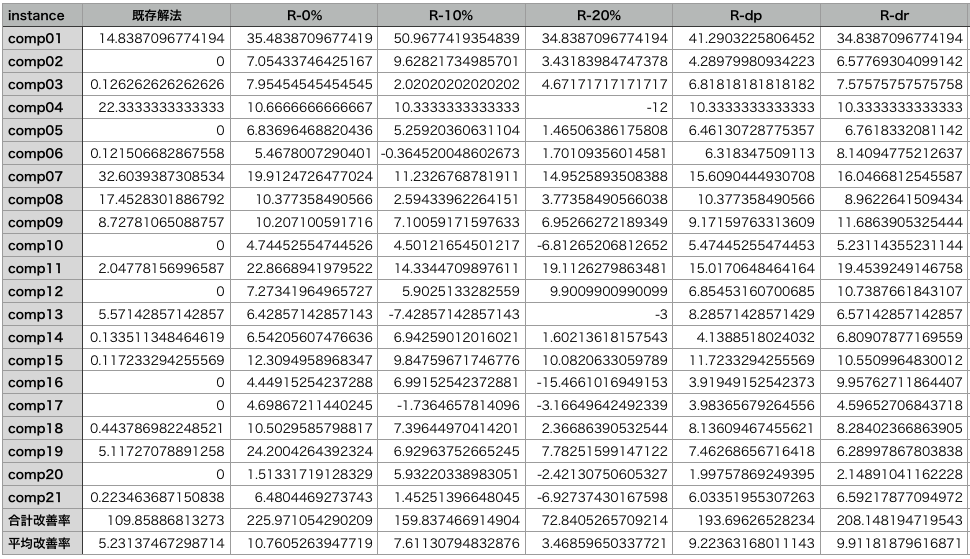
\includegraphics[width=12cm]{improve.png}
%\end{frame}
%
%\begin{frame}{初期解と既存の最良値を含めた比較}
%  \centering
% 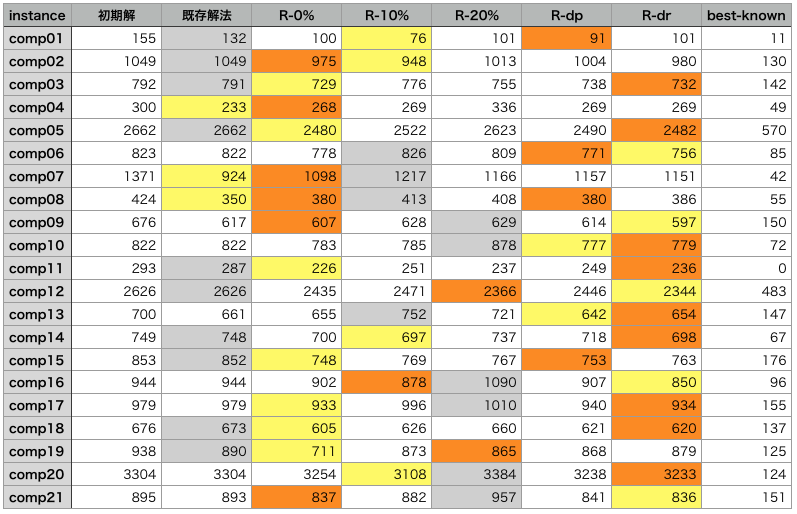
\includegraphics[width=12cm]{comp.png}
%\end{frame}

\end{document}

%%% Local Variables:
%%% mode: latex
%%% TeX-master: t
%%% End:
